\begin{figure}[ht]
\begin{subfigure}{.31\textwidth}
  \centering
  % include first image
  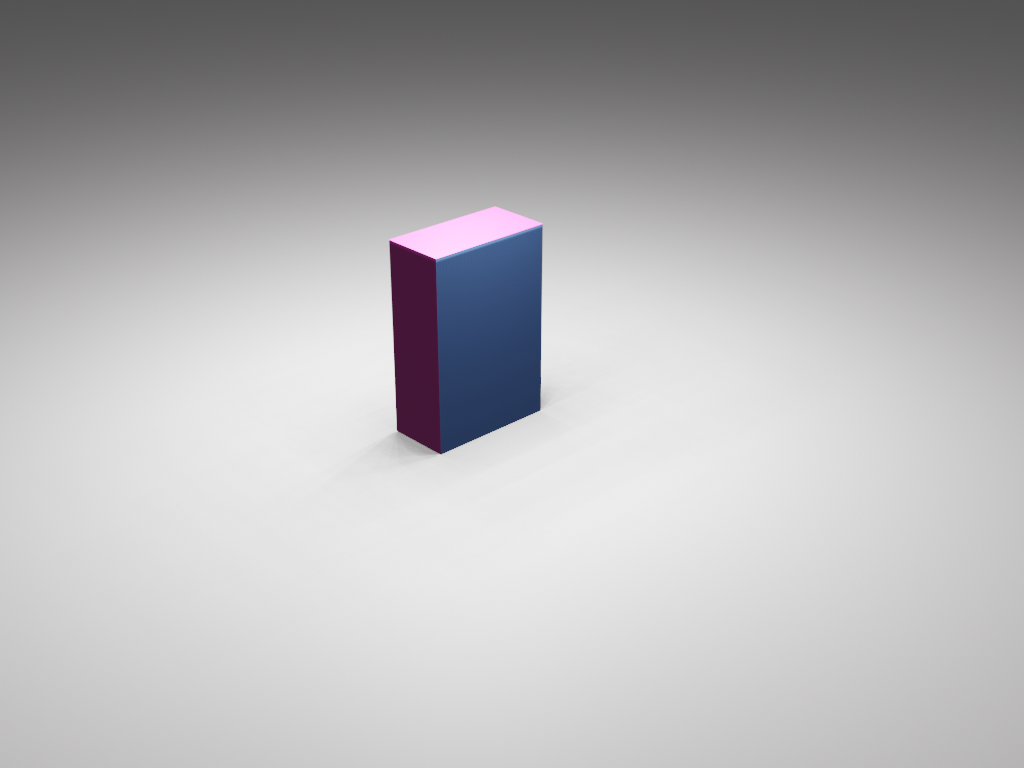
\includegraphics[width=.8\linewidth]{0001.png}  
  \caption{frame \# 1}
\end{subfigure}
\hfill
\begin{subfigure}{.31\textwidth}
  \centering
  % include second image
  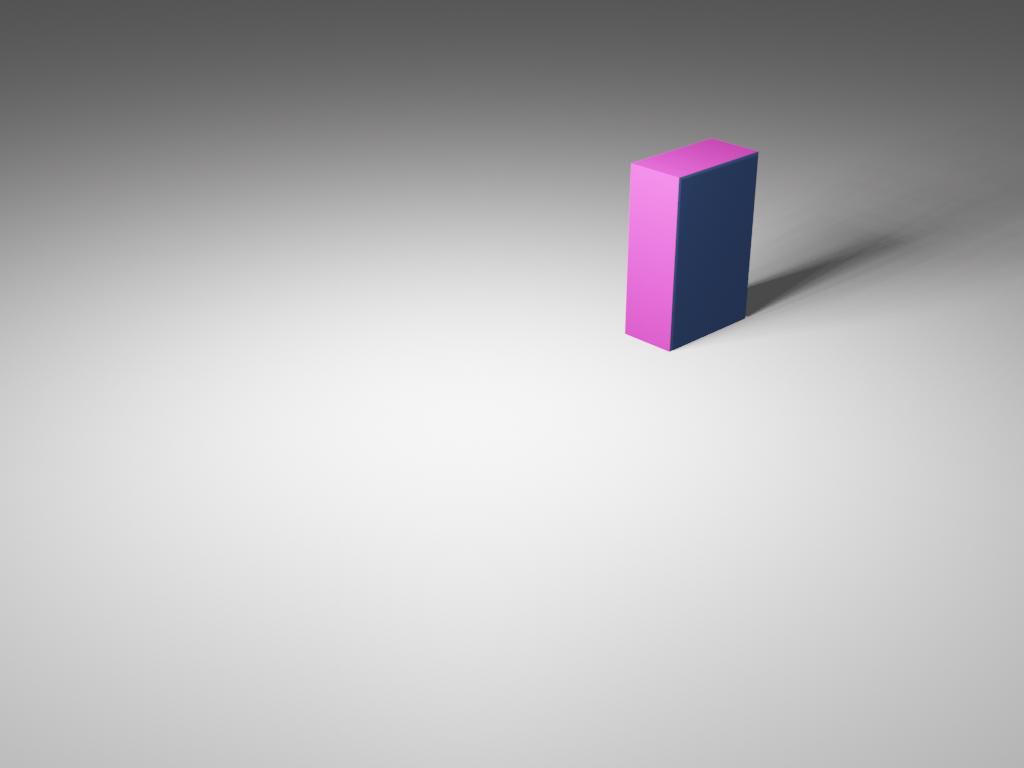
\includegraphics[width=.8\linewidth]{0100.png}  
  \caption{frame \# 100}
\end{subfigure}
\hfill
\begin{subfigure}{.31\textwidth}
  \centering
  % include second image
  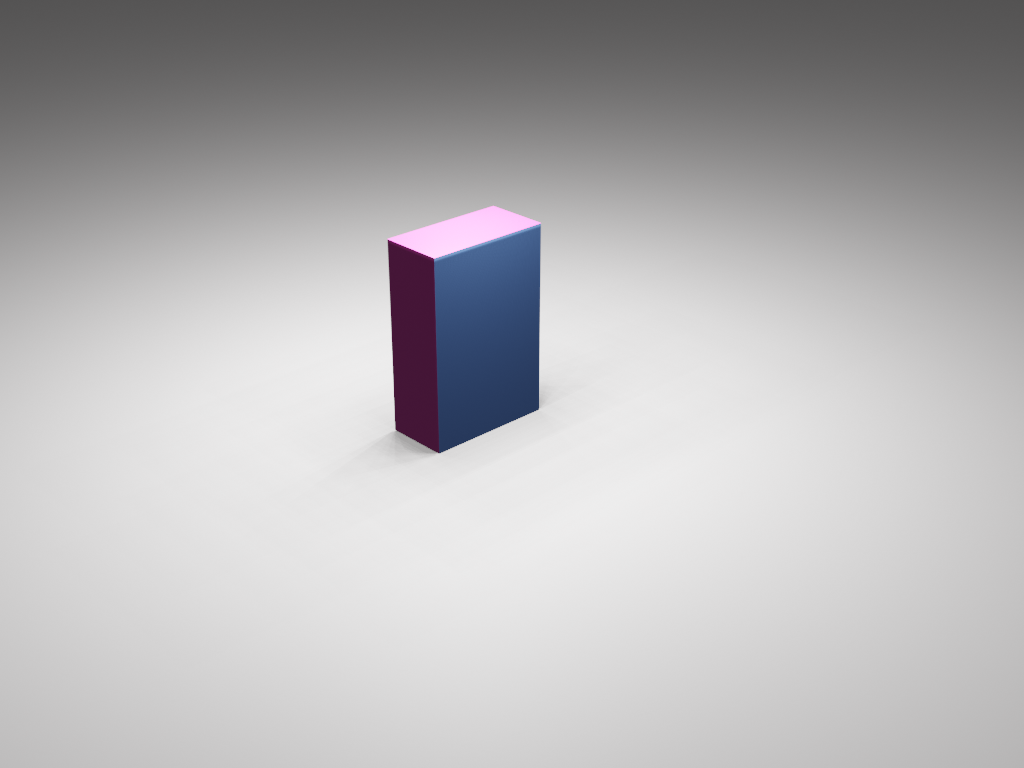
\includegraphics[width=.8\linewidth]{0200.png}  
  \caption{frame \# 200}
\end{subfigure} 
\\
\begin{subfigure}{.31\textwidth}
  \centering
  % include first image
  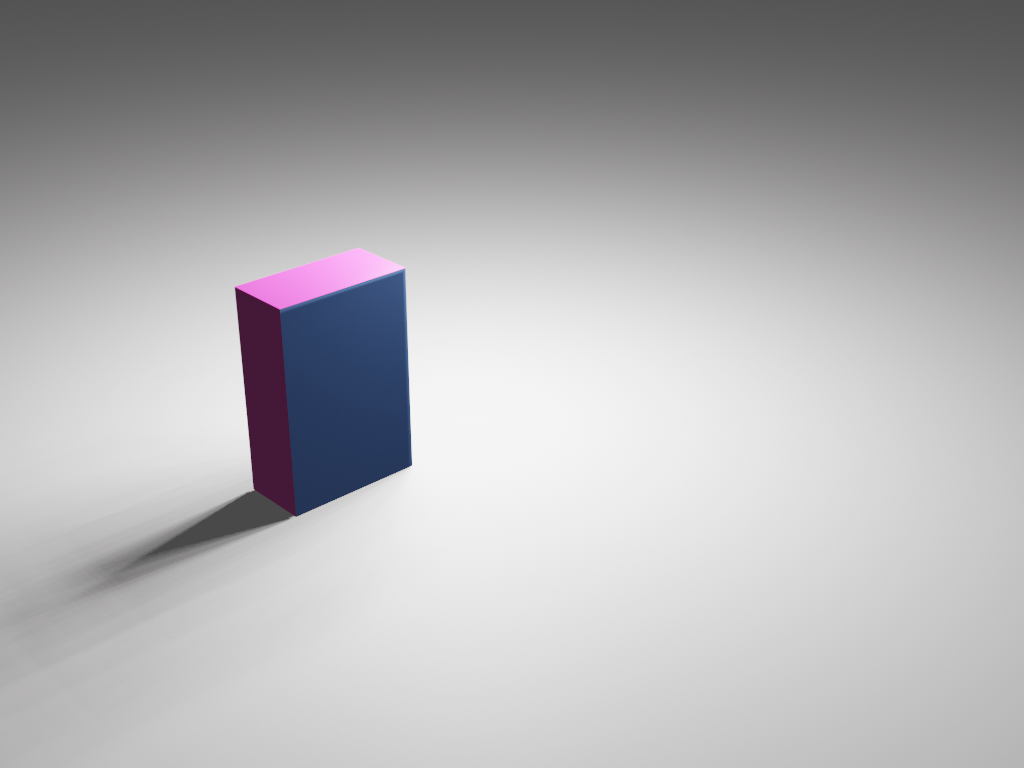
\includegraphics[width=.8\linewidth]{0300.png}  
  \caption{frame \# 300}
\end{subfigure}
\hfill
\begin{subfigure}{.31\textwidth}
  \centering
  % include second image
  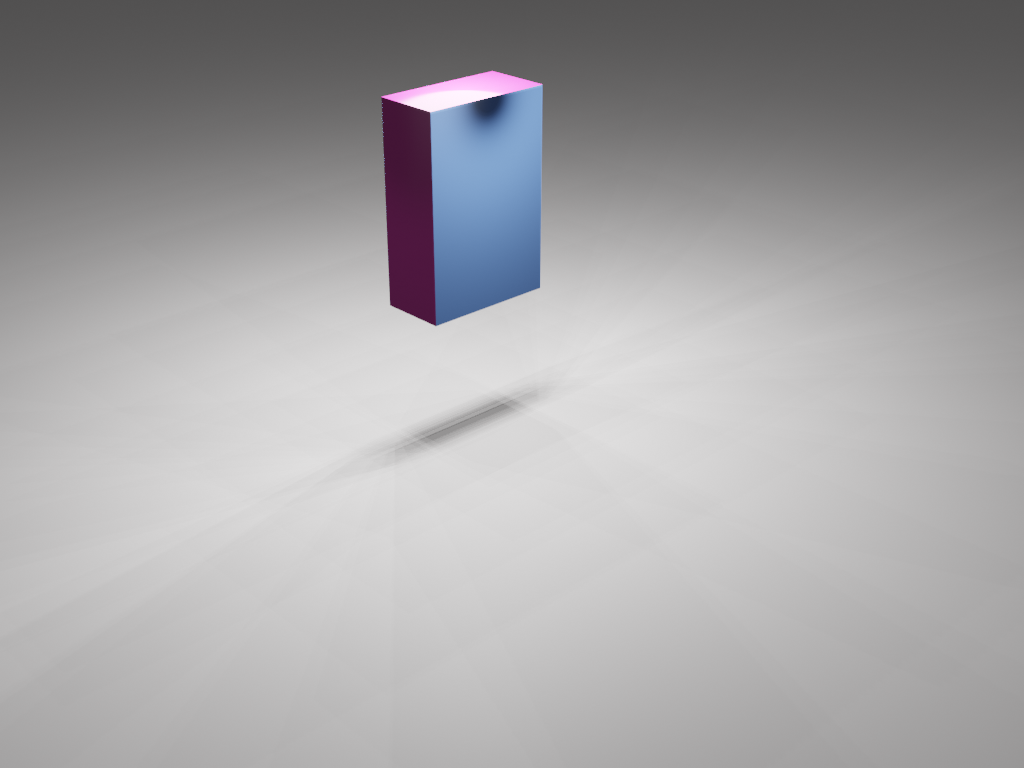
\includegraphics[width=.8\linewidth]{0400.png}  
  \caption{frame \# 400}
\end{subfigure}
\hfill
\begin{subfigure}{.31\textwidth}
  \centering
  % include second image
  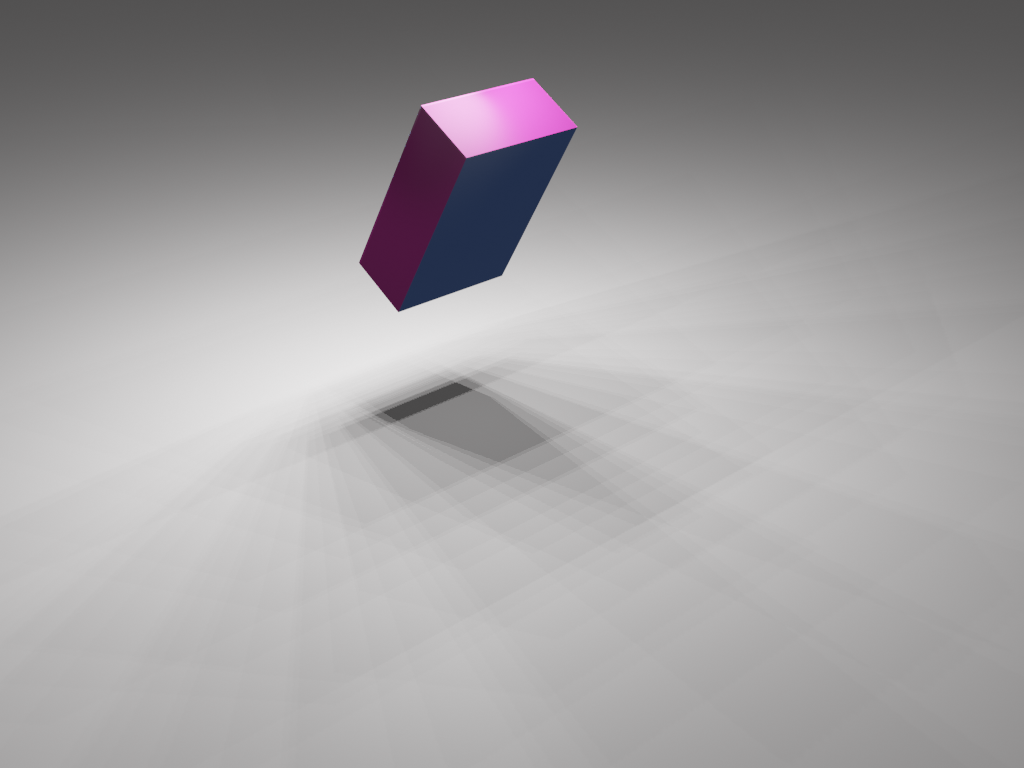
\includegraphics[width=.8\linewidth]{0500.png}  
  \caption{frame \# 500}
\end{subfigure} 
\\
\begin{subfigure}{.31\textwidth}
  \centering
  % include first image
  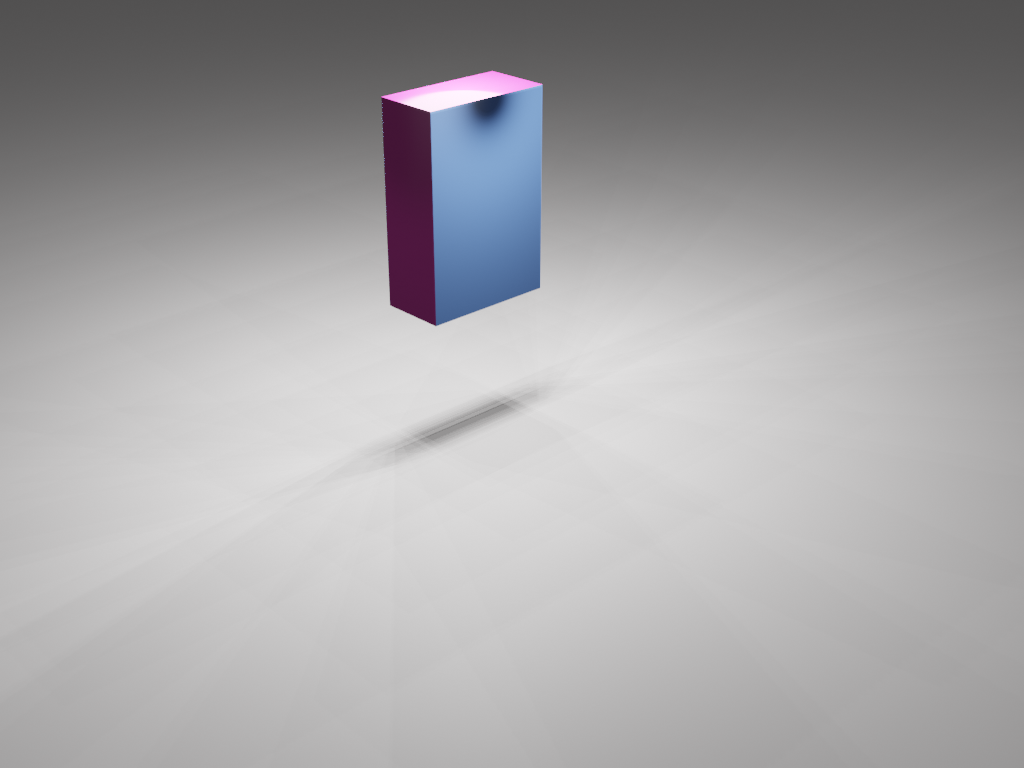
\includegraphics[width=.8\linewidth]{0600.png}  
  \caption{frame \# 600}
\end{subfigure}
\hfill
\begin{subfigure}{.31\textwidth}
  \centering
  % include second image
  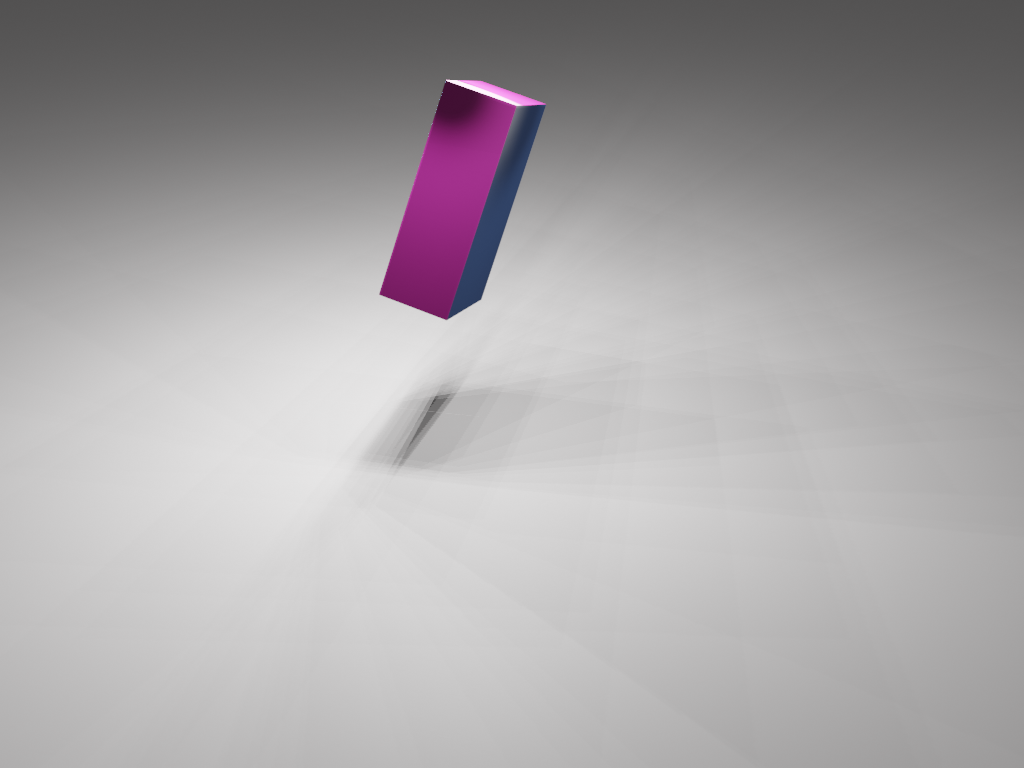
\includegraphics[width=.8\linewidth]{0700.png}  
  \caption{frame \# 700}
\end{subfigure}
\hfill
\begin{subfigure}{.31\textwidth}
  \centering
  % include second image
  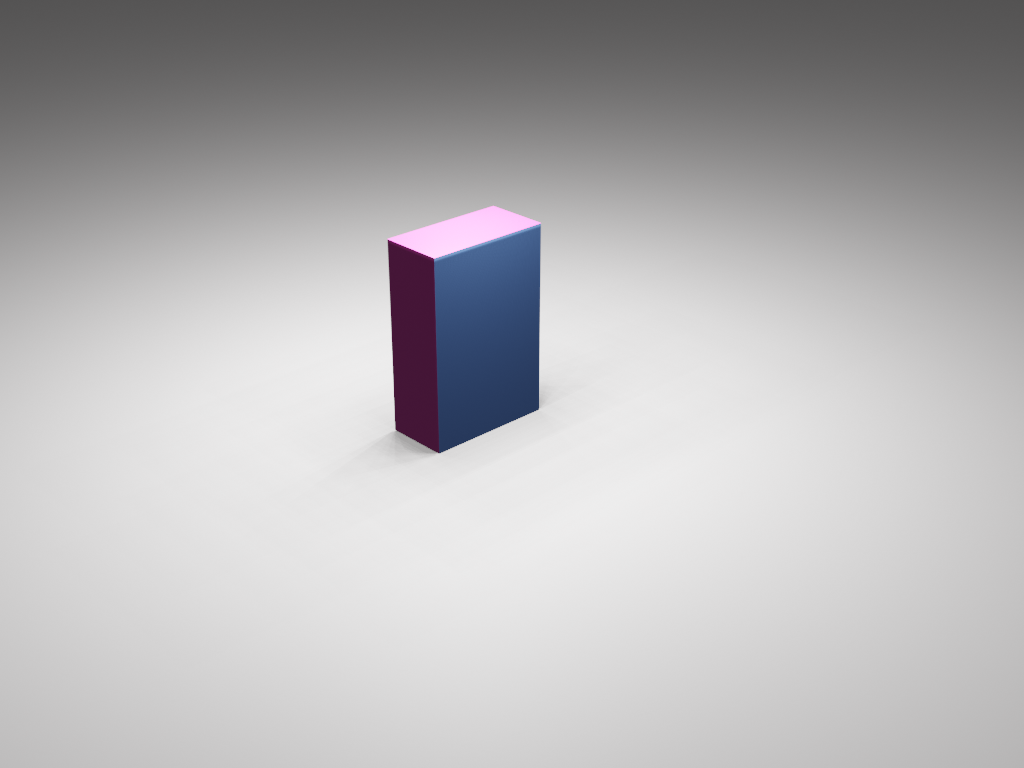
\includegraphics[width=.8\linewidth]{0800.png}  
  \caption{frame \# 800}
\end{subfigure} 
\caption{Samples Frames from the Synthetic Data Set}
\end{figure}